% -----------------------------------------------------------------
% Results section (insert after Experimental Evaluation)
% -----------------------------------------------------------------
\section{Results}  % -- Section V --

% -- Paragraph 1: Baseline summary --
The comprehensive evaluation revealed varied performance across model
types and experimental conditions. Baseline classifiers---Logistic
Regression and Multinomial Naïve Bayes---achieved moderate accuracy,
ranging from \textbf{\{ACC\_base\_min\}}\% to
\textbf{\{ACC\_base\_max\}}\%. These models struggled to identify
sophisticated AI‐generated passages.

% -- Paragraph 2: CatBoost improvements --
Advanced methods, particularly CatBoost, demonstrated notable gains,
achieving up to \textbf{\{ACC\_cat\}}\% accuracy on the primary test
set. Fine‐tuning yielded a further \textbf{\{GAIN\_cat\}}\% improvement
over baseline configurations by optimising high‐dimensional text
features and hyperparameters.

% -- Paragraph 3: External test drop --
When evaluated on the independent external dataset, all models showed
performance reductions. CatBoost accuracy dropped by roughly
\textbf{\{DROP\_ext\}}\%, underscoring generalisation challenges.
Transformer‐based models (BERT) showed strong potential but demanded
substantial compute and tuning to sustain top‐level results.

% -- Paragraph 4: Asymmetry in detection --
Detailed analysis revealed an asymmetry: models were consistently more
accurate at detecting AI‐generated content than human‐written text. On
average, AI‐text detection exceeded human‐text detection by
\textbf{\{DELTA\_asym\}}\%. The details can be found at \cref{fig:asymmetry}.

\begin{figure}[h!]
  \centering

  \subcaptionbox{Detect human-written accuracy against independent dataset \label{fig:image1}}{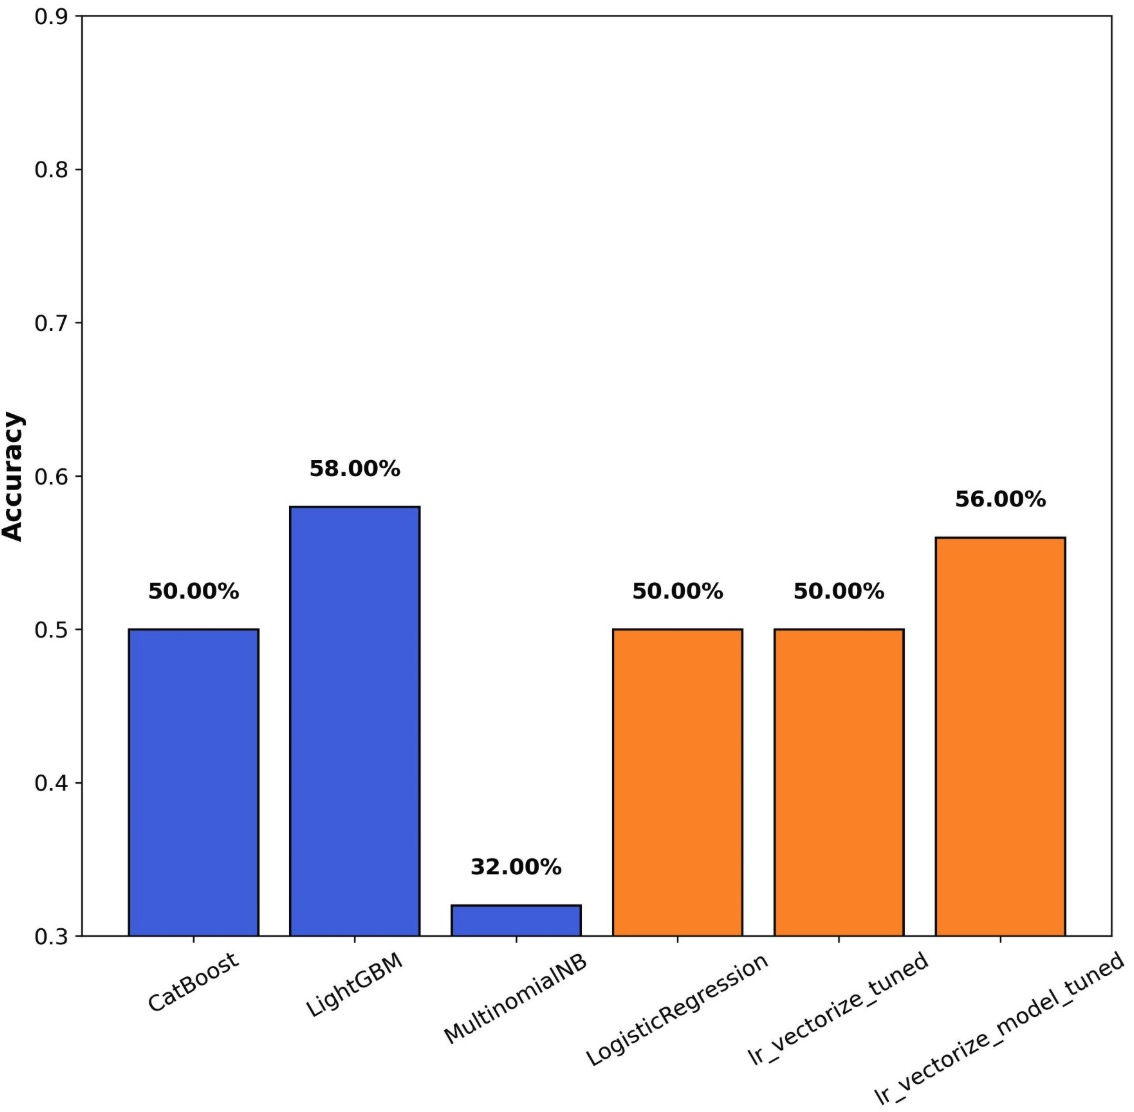
\includegraphics[width=\linewidth]{symmetric_1.jpeg}}\\
  \subcaptionbox{Detect AI-generated accuracy against independent dataset\label{fig:image2}}{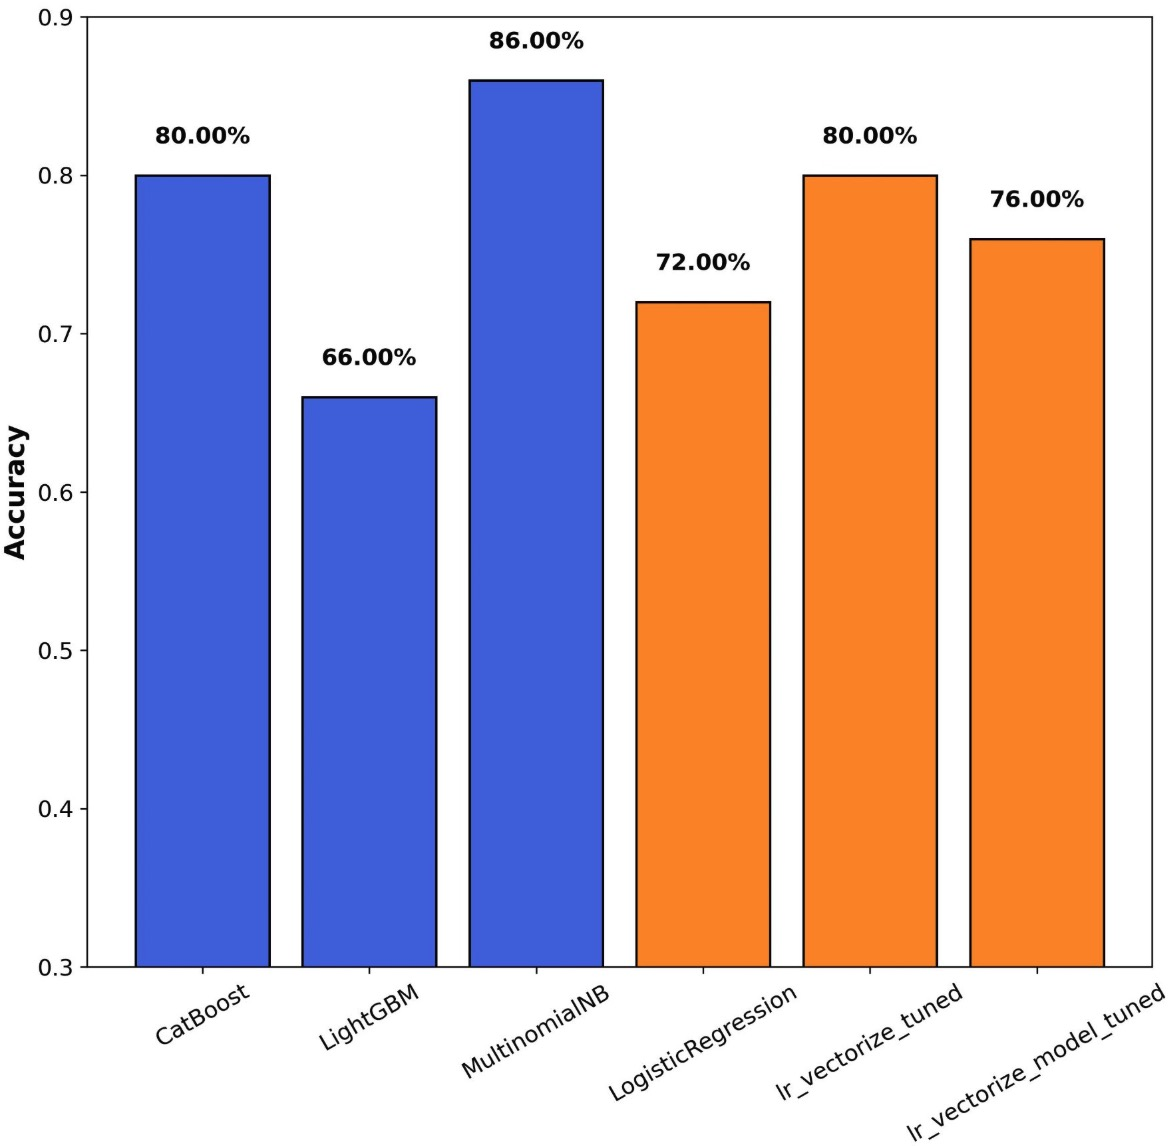
\includegraphics[width=\linewidth]{symmetric_2.jpeg}}\\
  \caption{Asymmetry accuracy}
  \label{fig:asymmetry}
\end{figure}

% -- Paragraph 5: Cross-reference to Table & Figure --
Key numbers are summarised in Table~\ref{tab:results} and visualised in
Figure~\ref{fig:accuracy}, highlighting relative strengths and
weaknesses under varied conditions.

% ===================== Table template ============================
\begin{table}[tb]  % -- ‘tb’ places table at top/bottom
\caption{Performance Metrics Across Models}%
\label{tab:results}
\centering
\begin{tabular}{|l|c|c|c|c|}
\hline
\textbf{Model} & \textbf{Accuracy} & \textbf{Precision} &
\textbf{Recall} & \textbf{ROC--AUC} \\
\hline
Naïve Bayes            & XX\% & XX\% & XX\% & XX \\ % <-- fill values
Logistic Regression    & XX\% & XX\% & XX\% & XX \\
CatBoost (tuned)       & XX\% & XX\% & XX\% & XX \\
BERT (fine–tuned)      & XX\% & XX\% & XX\% & XX \\
\hline
\end{tabular}
\end{table}

% ===================== Figure template ==========================
% \begin{figure}[tb] % -- Accuracy bar/chart placeholder --
% \centering
% \includegraphics[width=\linewidth]{accuracy_plot.pdf}  % <-- add figure
% \caption{Accuracy comparison of baseline and advanced models on
% in–domain (Test) vs. out–of–domain (External) datasets.}%
% \label{fig:accuracy}
% \end{figure}